 % -*- root: ../main.tex -*-
\chapter{RAFT}
	Come abbiamo visto nel capitolo precedente la struttura di una macchina a stati replicata è generalmente molto semplice. Questo è dato dal fatto che ogni singola state machine può essere decomposta in singoli \textbf{moduli} dedicati a uno \textbf{specifico scopo}.
	\begin{itemize}
		\item{\textit{Log Module}}
		\item{\textit{State Machine Module}}
		\item{\textit{Consensus Module}}
	\end{itemize}
	I moduli sono \textbf{semi-dipendenti} ossia comunicano tra di loro attraverso chiamate a procedure standard. Per esempio il modulo di log potrebbe esporre funzionalità dedicate all'appending o commiting di una serie di comandi, o ancora la state machine potrebbe mettere a disposizione un metodo per l'esecuzione di un determinato comando.\\
	In questo capitolo andremo a soffermarci maggiormente sul core-module di ogni SMR ossia il \textbf{modulo di consenso}; capiremo quali sono le sfide che un algoritmo di consenso deve affrontare e vedremo in dettaglio un'implementazione di un famoso algoritmo di consenso, \textbf{RAFT}.

	\section{Approcci al Consenso}
    % -*- root: ../../main.tex -*-
Esistono generalmente due approcci al problema del consenso:
\begin{itemize}
  \item{\textbf{Symmetric | Leader-less:}}
  In questa tipologia i server hanno tutti lo \textbf{stesso ruolo} e tutti lo stesso potere decisionale in qualsiasi momento.\\
  I \textbf{client} possono quindi \textbf{contattare} e fare richiesto verso \textbf{qualunque server} presente all'interno del cluster. 
  \item{\textbf{Asymmetric | Leader-base:}}
  In qualsiasi momento i server non hanno \textbf{mai} lo \textbf{stesso ruolo} e lo stesso potere decisionale. Esiste infatti sempre un server che si trova \textbf{in carica}, questo particolare server viene denominato \textbf{Leader}. Il leader gestisce solitamente tutte le operazioni del cluster, mentre gli altri server sono denominati \textbf{Servant} e portano a compimento le richieste del leader.\\
  In questo tipo di sistema i \textbf{client} possono \textbf{comunicare solamente con il leader}; nel caso in cui un client contatti un server diverso dal leader viene immediatamente \textbf{rediretto} al leader corrente.
\end{itemize}
Vedremo che RAFT implementa la seconda versione di consenso; questo garantisce all'algoritmo di essere estremamente più semplice dei suoi predecessori leader-less garantendo comunque lo stesso grado di safety.
  \section{L'algoritmo PAXOS}
    % -*- root: ../../main.tex -*-
Paxos è un algoritmo di consenso, non resistente a Byzantine Fault, sviluppato verso la fine degli anni ottanta e pubblicato nel 1998. Esso ha ricoperto il ruolo di algoritmo standard per decenni, venendo utilizzato in diversi ambienti, compreso quello didattico, poichè rappresenta un'ottima alternativa al commit a due fasi e a quello a tre fasi che si affidano entrambi ad un unico coordinatore che rappresenta un single point of failure. Esistono molte varianti di Paxos, ma la più usata si chiama \textit{Single Decree Paxos}.

In Paxos, i nodi possono assumere contemporaneamente uno o più dei seguenti ruoli:
\begin{itemize}
	\item \textbf{Proposer:} propone un valore su cui accordarsi a tutti gli acceptor;
	\item \textbf{Acceptor:} riceve le proposte dei proposer, decide se accettarle o meno e inoltra la propria risposta ai learner;  
	\item \textbf{Learner:} sulla base delle risposte ricevute, determina come valore vincitore quello scelto dalla maggioranza degli acceptor.
\end{itemize}


  \begin{figure}[H]
    \centering
    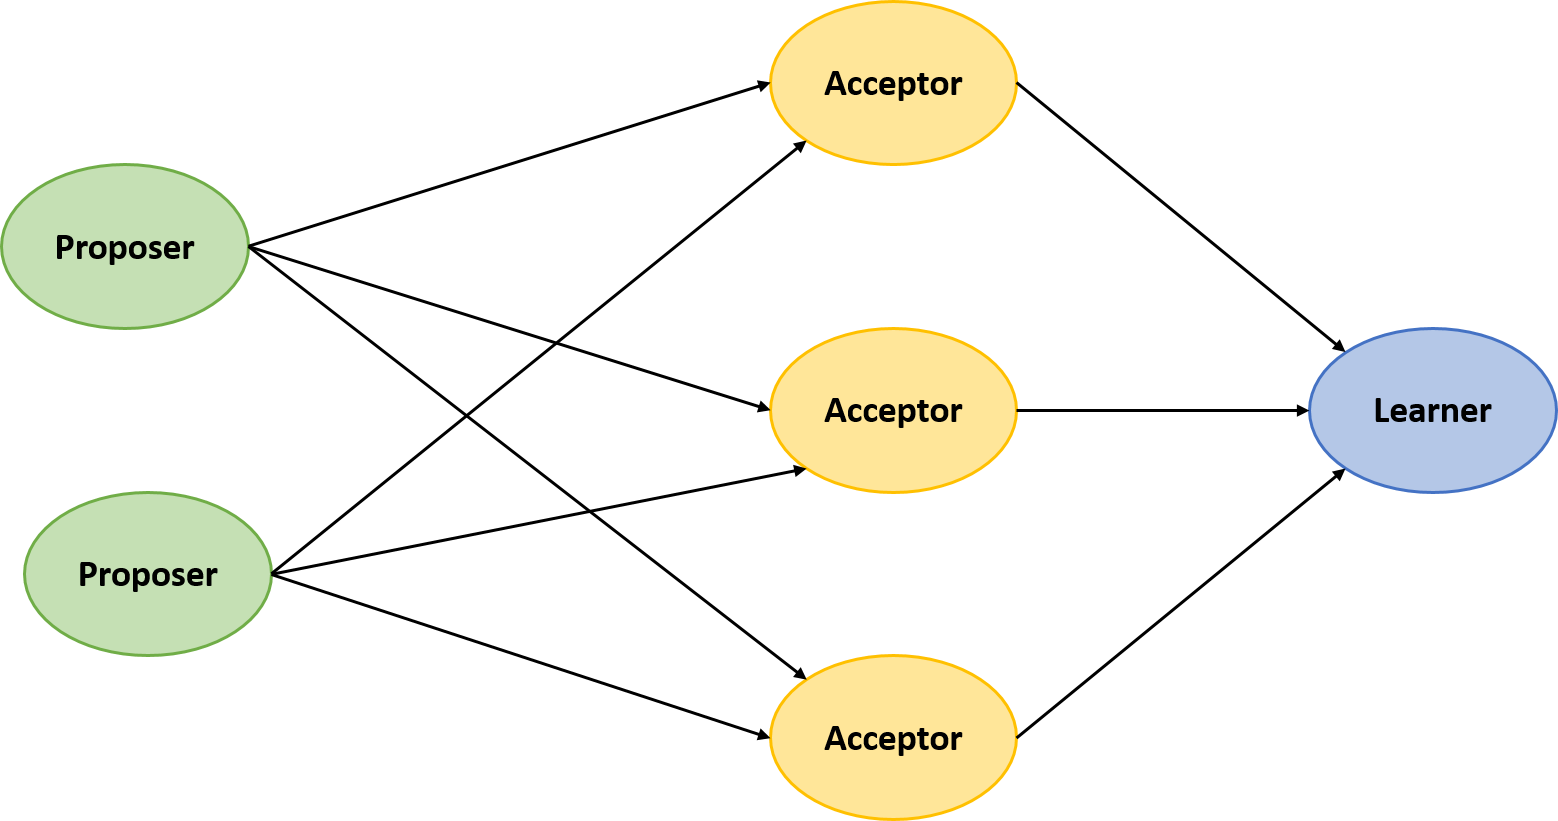
\includegraphics[width=0.90\columnwidth]{paxos/proposeAcceptLearn.png}
    \caption{Esempio di configurazione dei ruoli con due \textbf{proposer}, tre \textbf{acceptor} e un \textbf{learner} che sono rappresentati come nodi distinti per semplicità: nella realtà un nodo può ricoprire più di un ruolo alla volta.}
    \label{fig:figure 5}
  \end{figure}


Qualsiasi criterio si scelga per far decidere agli acceptor quale valore accettare, si incorre in casi di incorrettezza a meno di non utilizzare un approccio in due passi. 
Il raggiungimento del consenso si sviluppa quindi in due fasi.

\begin{enumerate}
	\item \textbf{Proposal:} in questa fase i proposer inviano una richiesta di \textit{prepare(n)} agli acceptor, dove \textit{n} è un \textit{proposal number} scelto in maniera tale che sia maggiore di ogni altro numero incontrato fino a quel momento. Gli acceptor ricevono le proposte e, per ognuna, controllano se il valore corrispondente è il maggiore in cui si siano imbattuti fino a quel momento: in caso affermativo, rispondono alla proposta impegnandosi a non accettare proposte precedenti, altrimenti la ignorano. Se un proposer riceve una risposta alla propria proposta dalla maggiorparte degli acceptor, passa alla seconda fase.
	
	\item \textbf{Accept:} in questa fase, il proposer invia il \textit{proposal number} e il \textit{value} tramite una richiesta \textit{accept(n,v)} rivolta a tutti gli acceptor. Se il proposer si vede ritornare come risposta il proprio \textit{proposal number} valore, allora la maggioranza degli acceptor ha concordato sul valore proposto, che quindi sarà quello scelto. Nel caso in cui ciò non accada, il proposer si vedrà arrivare un \textit{proposal number} maggiore del poprio, di conseguenza ricomincerà l'iter, tornando all'inizio della prima fase.
\end{enumerate}

  \begin{figure}[H]
    \centering
    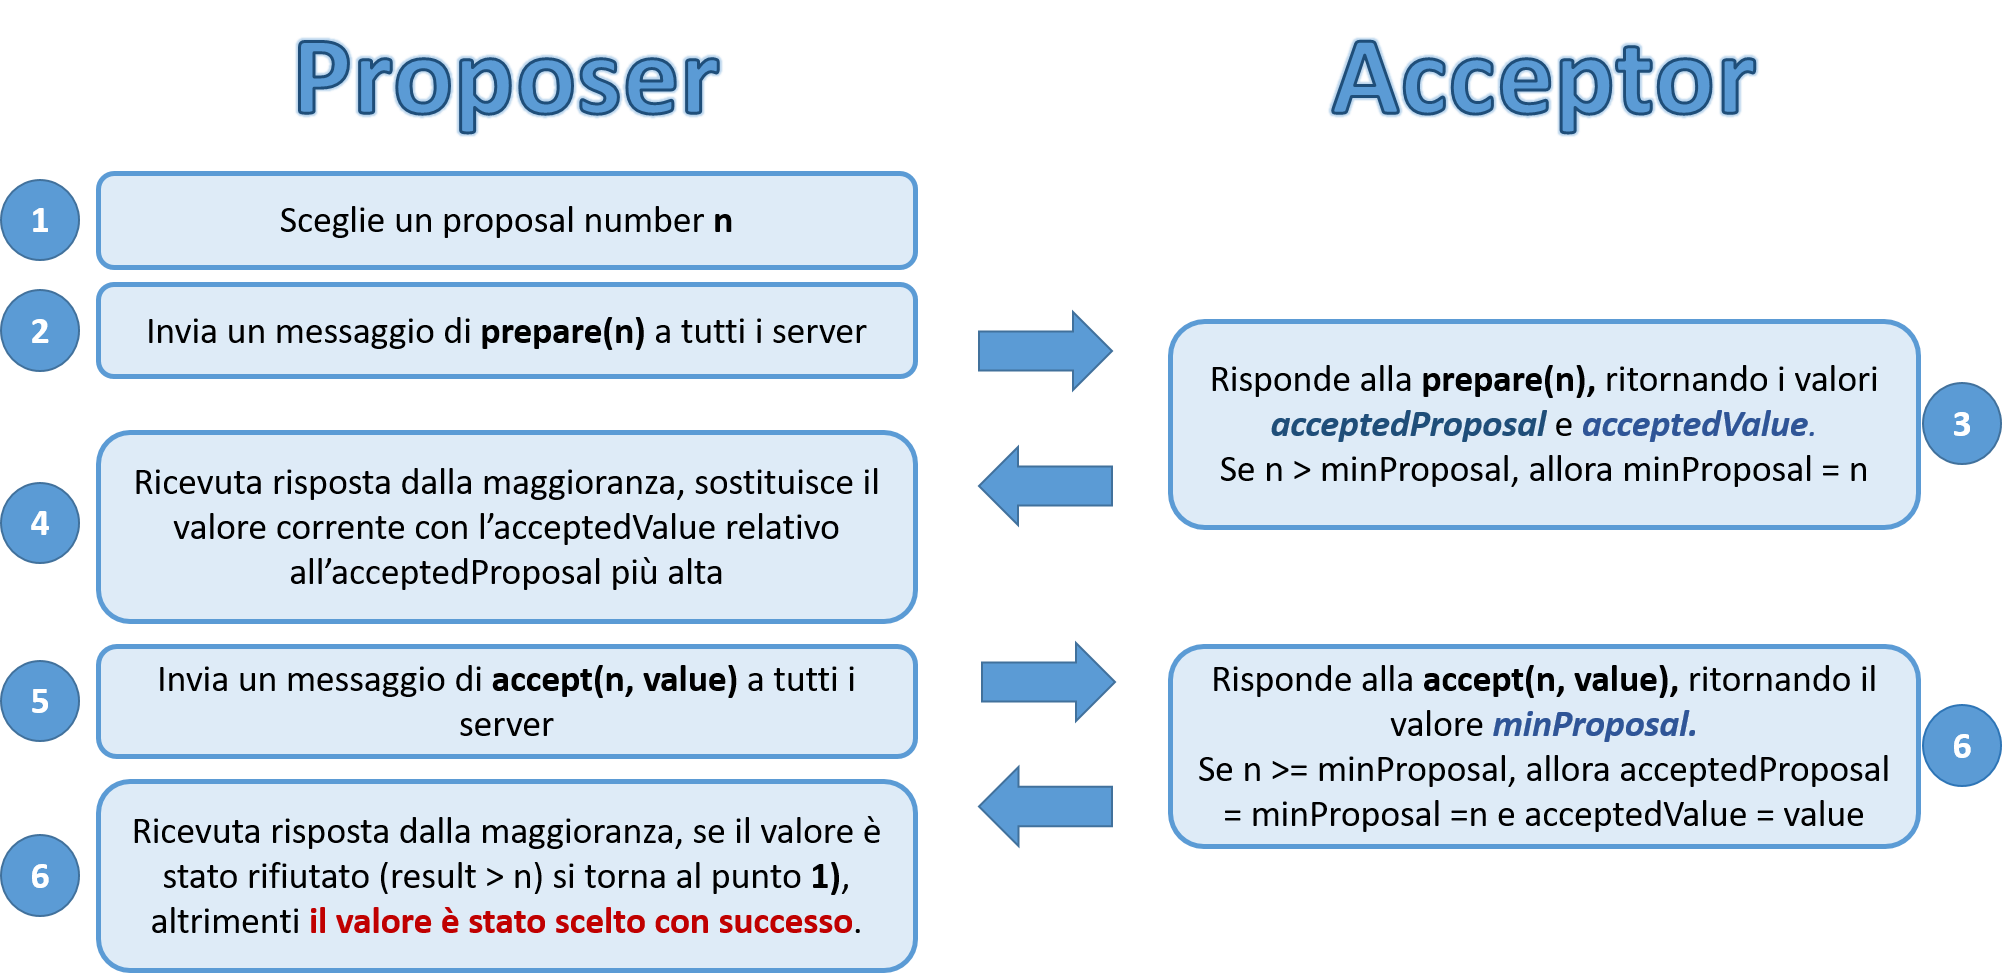
\includegraphics[width=0.90\columnwidth]{paxos/proposersAcceptorsInteraction.png}
    \caption{Schema riassuntivo delle interazioni tra proposer e acceptor, che non tiene conto, per semplicità, dei learner}
    \label{fig:figure 6}
  \end{figure}

L'algoritmo Paxos non è così semplice come potrebbe sembrare a una prima lettura, ma nasconde una serie di dinamiche complesse che non verranno analizzate in questo elaborato poichè è sufficiente un'infarinatura sul funzionamento generale di Paxos per capire in cosa differisce RAFT. 

Nonostante sia ancora largamente usato, l'algoritmo Paxos presenta dei difetti che RAFT ha provato a colmare:
\begin{itemize}
	\item \textbf{Difficoltà di comprensione:} la parte teorica e le dinamiche dell'algoritmo sono di difficile comprensione e spiegazione, come evidenziato anche dagli esperimenti condotti dagli autori di RAFT;
	
	\item \textbf{Difficoltà di implementazione:} anche una volta assimilata la parte teorica, è difficile applicarla. Quando si scende nei dettagli implementativi si va in contro a una confusione generale data dalla presenza di diverse interpretazioni, spesso errate.

	\item \textbf{Inefficienza:} prima che ci si possa accordare su un valore sono necessari almeno due round.

	\item \textbf{Valore unico:} il consenso viene raggiunto su un unico valore, per tutta la durata vitale del sistema.

	\item \textbf{Convergenza:} non è garantito che l'algoritmo converga, arrivando a una soluzione. L'unica garanzia è che se converge, il valore scelto sarà uno e uno solo.

\end{itemize}
	\section{RAFT Core}
    Quando si progetta un nuovo algoritmo è importante concentrasi sin da subito sui \textbf{metodi di valutazione} del risultato atteso. Generalmente i criteri utilizzati per la valutazione di algoritmi sono: 
    \begin{itemize}
      \item{\textbf{Correttezza:}}
      se l'algoritmo fornisce il risultato atteso in tutte le condizioni.
      \item{\textbf{Efficienza:}} 
      il numero di cicli di cpu o la quantità di memoria utilizzata dall'algoritmo. Solitamente questi due indicatori sono negativamente correlati, questo significa che cercando di ottimizzare un algoritmo sotto il profilo dei cicli di cpu si tenderà ad utilizzare più memoria.
      \item{\textbf{Concisione:}}
      un algoritmo è conciso quando le sue specifiche sono definite in modo preciso e chiaro.
    \end{itemize}
    Nel caso di RAFT, gli ideatori \textbf{Diego Ongaro e John Ousterhout} \cite[raftPaper]{raftPaper} \cite[ongaro:2014]{ongaro:2014} hanno deciso di usare un approccio inusuale, il loro scopo era prima di tutto quello della \textbf{understandability}\footnote{Un algoritmo pensato per essere comprensibile implicitamente obbliga l'autore a dover pensare in modo semplice e come sappiamo per il rasoio di Occham, la soluzione più veloce e comprensibile è generalmente quella migliore. Nel caso dei sistemi distribuiti questo è ancora più vero dato che in questo caso è importante sapere non solo che un algoritmo funzioni ma sopratutto perché funzioni.}.\\
    Nella progettazione di RAFT sono state applicate varie tecniche volte a garantire undestandability:
    \begin{itemize}
      \item{\textbf{Decomposizione del problema:}}
      tecnica che opera in modo simile al divide et impera degli algoritmi. Nella decomposizione il problema viene suddiviso parallelamente in problemi più piccoli e più semplici da risolvere.
      \item{\textbf{Minimizzazione dello spazio degli stati:}}
      la minimizzazione dello spazio degli stati può essere vista in modo molto naive come la riduzione del numero di istruzioni condizionali presenti. Questa procedura garantisce come piacevole conseguenza altre proprietà estremamente importanti:
      \begin{itemize}
        \item{\textbf{Gestione di problemi multipli con lo stesso meccanismo;}}
        \item{\textbf{Eliminazione degli stati speciali;}}
        \item{\textbf{Massimizzazione della coerenza e la consistenza;}}
        \item{\textbf{Minimizzazione del non-determinismo.}}
      \end{itemize}
    \end{itemize}
      \paragraph{RAFT in breve}
      RAFT implementa il \textbf{consenso} eleggendo prima di tutto un \texttt{leader} e fornendo allo stesso la totale responsabilità della gestione dei log replicati. Il leader una volta eletto \textbf{accetta} delle richieste dai \texttt{client}, le \textbf{replica} sugli altri server e \textbf{comunica} ai server quando è safe eseguire le stesse richieste nelle proprie state machines.\\
      L'esistenza del leader semplifica di molto l'algoritmo poiché garantisce un minor numero di stati del sistema. Nel caso in cui un leader fallisca o venga disconnesso verrà eletto un nuovo leader garantendo il progresso dell'algoritmo.

      \paragraph{RAFT e decomposizione}
      RAFT decompone il problema del consenso in tre problemi relativamente indipendenti:
      \begin{itemize}
        \item{\textbf{Leader Election:}}
         consiste nella \textbf{detection} di una \textbf{failure} da parte di un leader e nella definizione di un \textbf{protocollo di rielezione} che possa essere consistente.
        \item{\textbf{Log Replication:}}
        il leader deve essere l'unico server che può accettare comandi da parte di un client. Inoltre il leader deve assicurarsi di poter \textbf{replicare in modo safe} una entry presente nel log. 
        \item{\textbf{Safety:}}
        la proprietà di safety, chiave di RAFT, è data dalla State \textbf{Machine Safety Property}.
      \end{itemize}

		% -*- root: ../../../main.tex -*-
\subsection{Basics}
Un cluster RAFT può contenere vari server, solitamente cinque è il numero tipico, questo permette al sistema di tollerare due fallimenti.
  \subsubsection{Stati di un server}
  Abbiamo tre stati in cui si può trovare generalmente un server:
  \begin{itemize}
    \item{\textbf{Leader:}}
    In operazioni normali esiste esattamente \textbf{un solo leader} mentre i rimanenti sono followers. Quando il leader viene eletto allora esso ha \textbf{pieno potere} e tutti i rimanenti follower devono seguire i suoi ordini.\\
    Il leader solitamente ha due compiti fondamentali:
    \begin{itemize}
      \item{\emph{Gestione delle richieste da parte dei client}} 
      \item{\emph{Replicazione del log}}
    \end{itemize}
    \item{\textbf{Follower:}}
    I follower sono server totalmente \textbf{passivi}, essi intraprendono tre azioni fondamentali: 
    \begin{itemize}
      \item{\emph{Risposta alle richieste di leader e candidate}}
      \item{\emph{Redirection al leader delle richieste da parte dei client}}
      \item{\emph{Se non hanno più notizie dal leader da un po' allora diventano ``ansiosi'' e si convertono allo stato di candidate}}
    \end{itemize}
    \item{\textbf{Candidate:}}
    Lo stato di candidate è usato per \textbf{eleggere un nuovo leader}.
  \end{itemize}

  \begin{figure}[H]
    \centering
    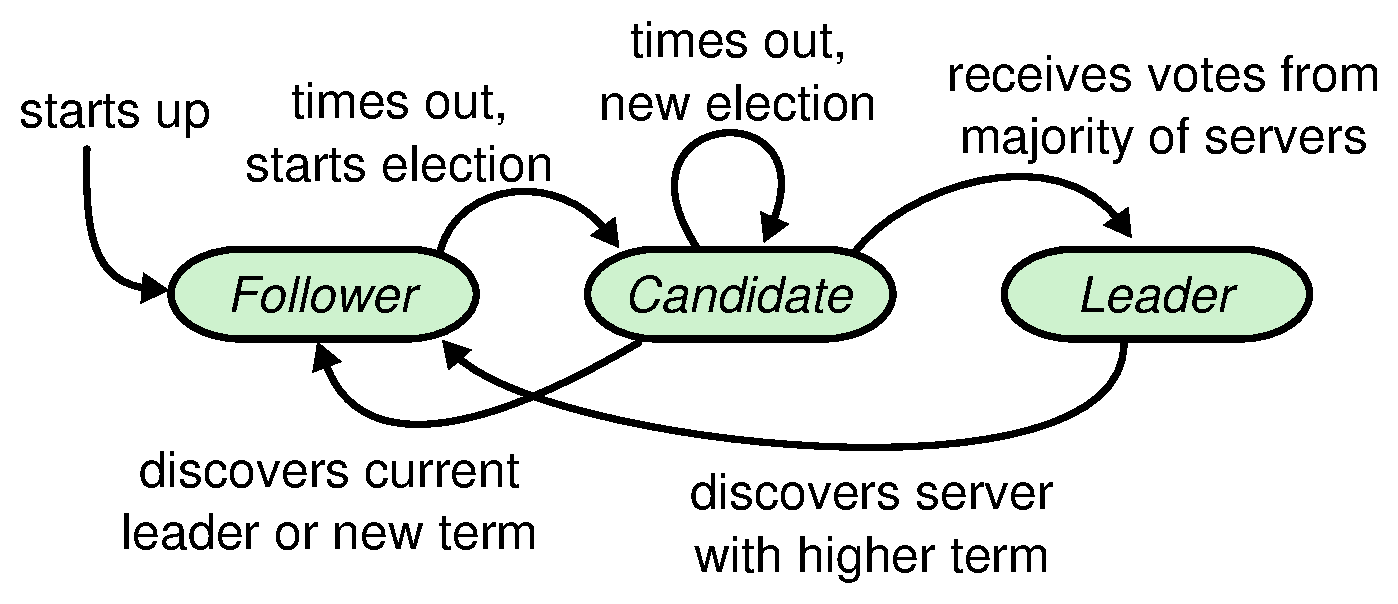
\includegraphics[width=0.90\columnwidth]{raft/followercandidateleader.pdf}
    \caption{Diagramma a stati che descrive il passaggio di stato dei singoli server}
    \label{fig:figure2}
  \end{figure}

  \subsubsection{Terms}
  Il tempo in RAFT è diviso in periodi di \textbf{lunghezza arbitraria} chiamati \textbf{terms}. I term godono di queste proprietà:
  \begin{itemize}
    \item{\textbf{Identificativo:}}
    A ciascun term è associato un numero in modo \textbf{incrementale} e \textbf{assoluto} nel tempo.
    \item{\textbf{Leader-centric:}}
    Ogni term parte con l'elezione di \textbf{uno e un solo leader}: se l'elezione ha successo allora il candidate eletto avrà potere per tutta la durata del term. Può capitare che più candidate provino a diventare leader nello stesso instante: in questo caso il risultato della votazione premierà un solo candidate. RAFT garantisce che non ci sia \textit{più di un leader per term}.
    \item{\textbf{Leader-less:}}
    In alcuni casi può capitare che nessun leader emerga, questo avviene perché nella votazione non è stata ottenuta una maggioranza assoluta. In questo caso si dice che è avvenuto un \textbf{split-vote} e al fine di garantire safety \textit{nessun leader può essere eletto}.\\
    In questo caso l'algoritmo considererà l'elezione come \textbf{failed} e verrà aperta immediatamente una \textbf{nuova elezione}.
    \item{\textbf{Term come logical clock:}}
    I term in RAFT hanno uno scopo molto più generale oltre al contesto dell'elezione: essi agiscono come \textbf{logical clock} \cite[Lamport:1978]{Lamport:1978} garantendo un concetto logico di tempo e permettendo ai server di accorgesi quando sono in possesso di \textbf{informazioni obsolete}.
  \end{itemize}
  
  \begin{figure}[H]
    \centering
    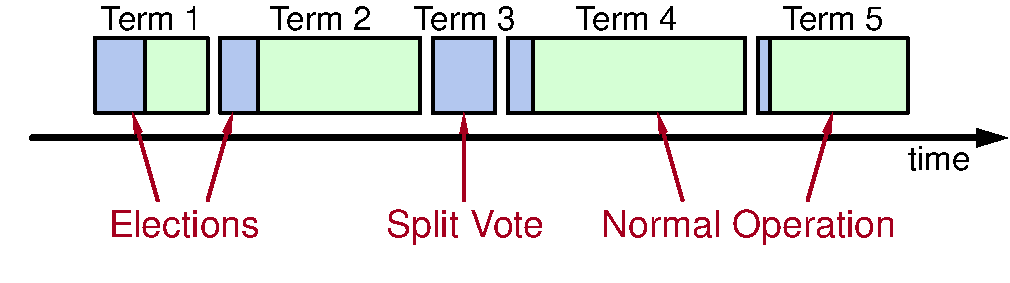
\includegraphics[width=0.80\columnwidth]{raft/terms}
    \caption{Un term è un priodo di tempo che parte con l'elezione di un nuovo leader e termina con la fine del suo "regno".}
    \label{fig:figure3}
  \end{figure}

    \paragraph{Identificazione di informazioni obsolete}
    Non esiste in RAFT un concetto di stato/term globale ma ogni \textbf{server vede}, in un \textbf{dato istante}, una \textbf{parte del sistema} e non è detto che sia lo stesso per tutti.\\
    L'identificazione di informazioni obsolete avviene in modo molto semplice:
    \begin{enumerate}
      \item Ogni server contiene al suo interno le informazioni sul \textbf{term attuale} che ovviamente può incrementare nel tempo in modo monotono.
      \item Nel momento in cui avviene una comunicazione ogni server \textbf{include} nel proprio \textbf{messaggio} anche le informazioni sul \textbf{proprio term}.
      \item Nel caso in cui un server si accorga di avere un term troppo obsoleto \textbf{aggiorna} immediatamente il proprio \textbf{term} con quello più \textbf{recente}.
      \begin{itemize}
        \item Se il server si trova nello stato di leader allora esso \textbf{regredisce} immediatamente \textbf{a follower}
      \end{itemize}
      \item Se un server riceve messaggi con \textbf{term obsoleti} questi vengono immediatamente \textbf{rifiutati}.
    \end{enumerate}
  \subsubsection{Tipologie di Messaggio | Remote Procedure Calls}
  Al fine di massimizzare la comprensibilità RAFT definisce solamente due tipologie di messaggio:
  \begin{itemize}
    \item{\textbf{Request Vote:}}
    I messaggi di questo tipo sono spediti dai \textbf{candidates} durante il processo di \textit{leader election}.
    \item{\textbf{Append Entries:}}
    Questi messaggi sono usati dai \textbf{leaders} con tre scopi fondamentali:
    \begin{itemize}
      \item{\emph{Log replication di una o più entries}}
      \item{\emph{Heartbeat con lo scopo di evitare che i follower possano iniziare una nuova elezione}}
      \item{\emph{Trasferimento di Snapshot tra i vari server}}
    \end{itemize}
  \end{itemize}
  \subsubsection{Gestione del tempo}
  L'unica nozione di tempo logico è quella di term, non ci sono \textit{clock condivisi} fra le macchine. Esiste una nozione di tempo implicita che garantisce il progresso: essa risiede nel concetto di \textbf{timeouts}.

  \subsubsection{Scalabilità}
  Per il fatto che un algoritmo di consenso necessita della maggioranza dei server per effettuare qualsiasi operazione il concetto di \textbf{scalabilità viene meno}. L'unico modo di garantire scalabilità consiste nel \textbf{partizionare} i server in \textbf{più cluster} e usare un algoritmo di consenso fra cluster: questo è il caso dei sistemi di storaging di elevate dimensioni come Megastore, Spanner e Scatter.
		% -*- root: ../../../main.tex -*-
\subsection{Leader Election}
\label{Leader Election}
In un dato term, tutte le \textit{operazioni di replicazione} del log sono affidate ad un server che ricopre il ruolo di \textit{leader}. Al fine di accordarsi in maniera safe su un unico leader è necessario applicare un protocollo di elezione robusto.  

	\subsubsection{Candidatura}
	Ogni elezione ha inizio nel momento in cui uno o più server si candidano come aspiranti leader.

	\begin{enumerate}
		\item{\textbf{Stato iniziale:}}	ogni server inizialmente si trova nello stato di follower e vi resta fintantochè riceve nuovi messaggi dall'attuale server leader.
		\item{\textbf{Heartbeat:}} il leader, periodicamente, invia un messaggio detto di \textit{heartbeat}\footnote{come heartbeat vengono utilizzati i messaggi di tipo AppendEntries che, nel caso in cui non ci sia effettivamente una entry da appendere, vengono lasciati vuoti.} 
		per comunicare ai suoi follower che è ancora in funzione.
		\item{\textbf{Timeout:}} i server \textbf{follower} mantengono internamente un \textbf{timer randomico} che si resetta ogni volta che viene ricevuto un messaggio dal leader. La durata di questo timer viene chiamata \textit{election timeout}.		
		\item{\textbf{Inizio candidatura:}} allo scadere del timer, il follower considera il leader assente e si propone come leader effettuando un \textbf{cambiamento di stato} da follower a candidate e dando inizio a una \textbf{nuova leader election}.
	\end{enumerate}


Quando una \textit{Leader Election} ha inizio il follower esegue i seguenti passaggi:

\begin{enumerate}
	\item{\emph{Incrementa di uno il proprio term}}
	\item{\emph{Cambia il proprio stato in candidate}}
	\item{\emph{Vota per sè stesso}}
	\item{\emph{Invia in broadcast un messaggio di tipo ``Request Vote'' affinchè gli altri membri del cluster possano votarlo}}
\end{enumerate}
 
A questo punto possono verificarsi i seguenti tre scenari:
\begin{enumerate}
	\item{\textbf{Il candidate vince l'elezione:}} questo accade quando il numero di voti ricevuti dagli altri membri del cluster (compreso il proprio) raggiunge la maggioranza.\\
	A questo punto \textit{cambia il suo stato in \textbf{leader}} e invia un \textbf{heartbeat}, con lo scopo di controllare il cluster evitando che si inneschino nuove candidature.

	\item{\textbf{Un altro candidate vince l'elezione:}} questo può accadere se ad esempio i due si candidano a poca distanza l'uno dall'altro. A questo punto il \textbf{Candidate} che ha perso, riceverà un messaggio dal nuovo \textbf{Leader} e tornerà \textbf{Follower}.
	
	\item Nessuno vince le elezioni: la contemporanea presenza di più \textbf{Candidate} può portare a uno \textit{Split Vote}, ovvero una situazione in cui nessuno dei \textbf{Candidate} ottiene la maggioranza dei voti. In questo caso il term termina senza aver avuto un leader e viene dato inizio al term successivo.
\end{enumerate}
Ogni \textbf{Follower} del cluster può avere una sola preferenza di voto per term, questo garantisce che per un dato term ci sia al più un solo \textbf{Leader}. \\
Quando un \textbf{Candidate}, durante le elezioni, riceve un messaggio da un \textbf{Leader}, ne verifica il term: se questo è inferiore al proprio, non riconosce il \textbf{Leader} come legittimo; se il term è maggiore, passa allo stato di \textbf{Follower}.
D'altra parte, il \textbf{Leader}, quando riceverà la \textit{Request Vote}, notando che il suo term è minore, tornerà allo stato di \textbf{Follower} e invierà il proprio voto.
\\
Ogni \textbf{Candidate} mantiene internamente un timer randomico che viene inizializzato ad un valore che oscilla tra un massimo e un minimo, come accade per i \textbf{Follower}.
Questo timer, quando innescato, viene impostato ad un nuovo valore e fa si che il \textbf{Candidate} incrementi il suo term e invii nuovamente delle \textit{Request Vote} a tutto il cluster, come se si fosse ricandidato. Questo meccanismo minimizza la possibilità che si verifichino consecutivamente più \textit{Split Vote}.


\begin{figure}[H]
	\centering
	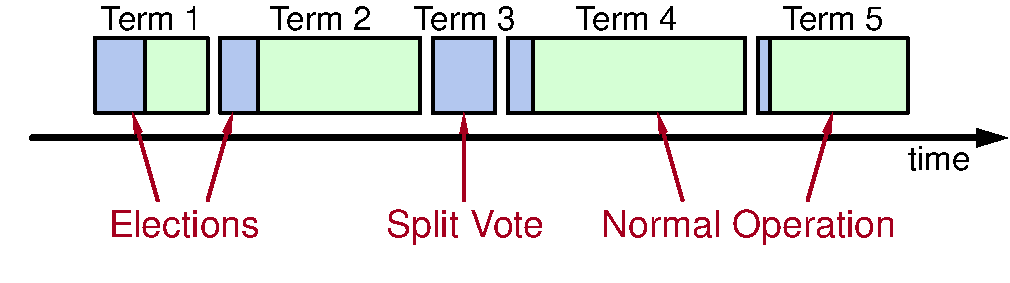
\includegraphics[width=0.80\columnwidth]{raft/terms}
	\caption{Un term è un priodo di tempo che parte con l'elezione di un nuovo leader e termina con la fine del suo "regno". 
		Un term attraversa normalmente due fasi: durante la prima, evidenziata in blu, i server eleggono il proprio leader; durante la seconda, evidenziata in verde, si svolgono le normali operazioni coordinate dal leader in carica.
		Non è possibile che due candidati ottengano la maggioranza all'interno dello stesso term, tuttavia è possibile che l'elezione si concluda in parità, come nel Term 3 in figura. In questo caso il term si conclude e ne inizia uno nuovo in cui si avvia una nuova elezione.}
	\label{fig:figure3}
\end{figure}


\begin{figure}[H]
	\centering
	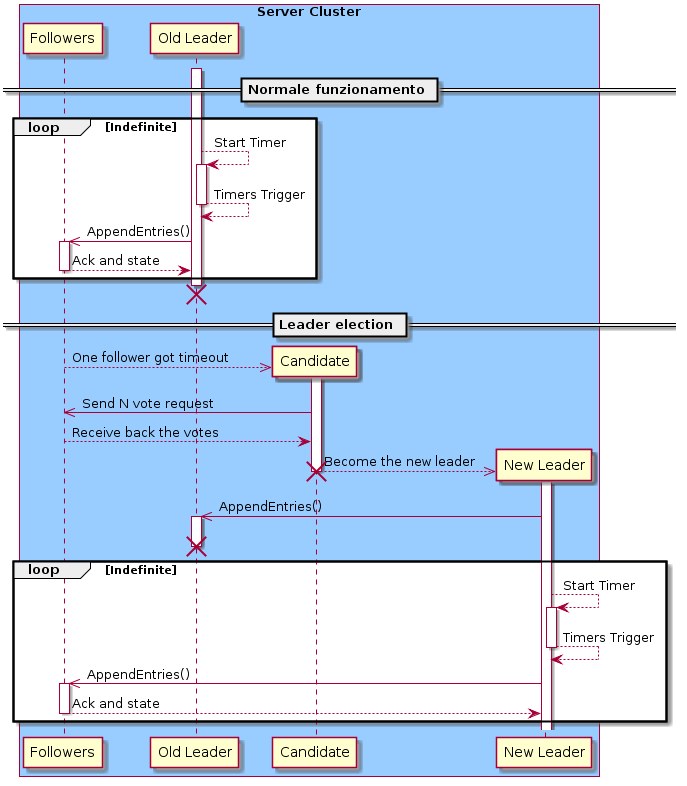
\includegraphics[width=0.80\columnwidth]{seqDiagrams/LeaderElection}
	\caption{Uno scenario semplificato in cui viene mostrata una \textit{Leader Election}. Il vecchio \textbf{Leader} inizialmente svolge correttamente le sue mansioni, divulgando periodicamente i propri \textit{heartbeats}; successivamente non riesce più a svolgere le sue attività. Prima o poi, non ricevendo più notizie dal leader, uno dei \textbf{Follower} vedrà scadere il proprio timer. Diventato \textbf{Candidate}, esso procederà a inviare le \textit{Vote request} a tutti i follower del cluster. Ricevuta la maggioranza dei voti verrà eletto \textbf{Leader} e ripristinerà il normale funzionamento del cluster. Il vecchio \textbf{Leader} quando tornerà on-line riceverà un AppendEntry e tornerà allo stato di \textbf{Follower}.}
	\label{fig:figure4}
\end{figure}



		% -*- root: ../../../main.tex -*-
\subsection{Normal Operation | Log Replication}
\label{Log Replication}
Prima di proseguire con la descrizione della seconda fase dell'algoritmo (\textit{log replication}) è bene fornire una definizione completa della struttura del log.
  \subsubsection{Struttura del Log}
  In RAFT ogni server, compreso il leader, mantiene una copia personale del log. Ogni singolo log è strutturato in questo modo:
  \begin{itemize}
    \item{\emph{\textbf{Entry:}}}
    \emph{Ogni log è suddiviso in celle chiamate \textbf{entry} identificate da un \textbf{indice} che ne indica la \textbf{posizione} nel log}
    \item{\emph{Ogni singola entry si compone di due campi:}}
      \begin{itemize}
        \item{\emph{\textbf{Comando:}}}
        \emph{Un comando o una procedura sulla quale tutte le macchine presenti nel cluster devono trovare un accordo.}
        \item{\emph{\textbf{Term:}}}
        \emph{Rappresenta il term relativo a quando la entry è stata aggiunta al log. Ciò sta a significare che la entry è stata aggiunta dal leader al suddetto term.}
      \end{itemize}
    \item{\emph{\textbf{Memorizzazione:}}}
    \emph{Ogni log è memorizzato in una memoria locale in modo da permettere resistenza ai crash del server.}
    \item{\emph{\textbf{Commited entry:}}}
    \emph{Nel momento in cui una entry è replicata sulla maggioranza dei server allora si considera \textbf{committed} e può essere esguita dalle state machines.}
  \end{itemize}
  \begin{figure}[H]
  	\centering
  	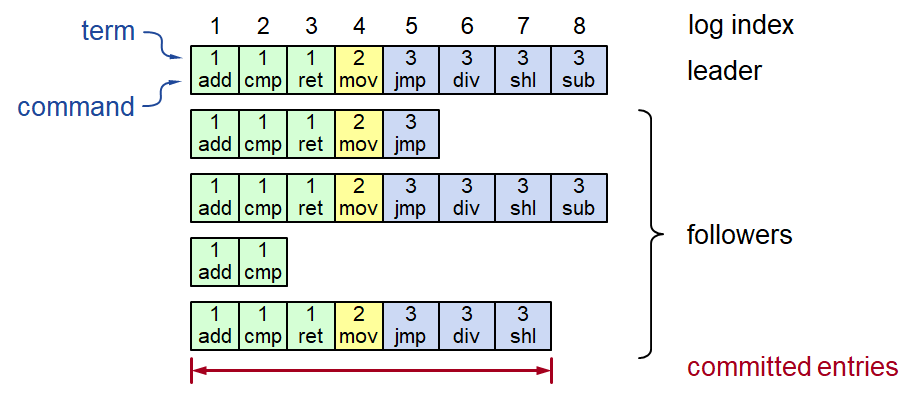
\includegraphics[width=0.99\columnwidth]{raft/logStructure}
  	\caption{Nell'immagine possiamo vedere che la entry n.7 è commited poiché è replicata sulla maggioranza dei server. Entry n.8 non può essere commited poiché è replicata solo su 2/5 dei server.}
  	\label{fig:figure6}
  \end{figure}

  \subsubsection{Log Replication}
  Una volta eletto correttamente, il leader inizia a servire tutte le richieste che provengono dai client. La log replication in situazioni normali procede come segue:
  \begin{enumerate}
    \item{\emph{Il leader \textbf{appende} il comando al proprio log.}}
    \item{\emph{Il leader invia dei messaggi di tipo \textbf{AppendEntries} ai followers.}}
    \item{\emph{Quando la \textbf{maggioranza dei follower} comunica al leader di aver replicato il log allora la entry può essere \textbf{committed}. Nel caso di mancate risposte il leader attende riprovando a inviare la entry.}}
    \item{\emph{Il leader \textbf{passa il comando} alla propria state machine che lo \textbf{esegue}, il \textbf{risultato} viene poi ritornato al client.}}
    \item{\emph{Il leader inoltre comunica ai followers il commitment e finalmente li abilita alla esecuzione del comando.}}
  \end{enumerate}
  Il leader mantiene traccia dell'ultima entry che è stata validata, e include il suo indice e term in tutte le \textit{AppendEntries} (inclusi gli \textit{heartbeats}). Cosi facendo i followers potranno rimanere allineati riuscendo cosi ad eseguire in modo tempestivo il comando non appena riconoscono che esso è stato committato.

  \subsubsection{Log Matching Property}
  \label{Log Matching}
  La proprietà di log matching garantisce che:
  \[
    \begin{multlined}
    \emph{\textbf{Se una entry è committed}}\\
    \emph{\textbf{allora anche tutte 
    le entry precedenti lo saranno.}}
    \end{multlined}
  \]
  Questa proprietà deriva da queste sotto-proprietà:
  \begin{itemize}
    \item{\emph{Se due log hanno un entry con lo stesso index e stesso term, allora quell'entry contiene lo stesso comando(sono identiche)}}.
    \item{\emph{Se due \textit{entry} in log diversi hanno lo stesso index e lo stesso term, allora anche tutte le loro precedenti entry sono identiche tra i due log}}.
  \end{itemize}
  La prima proprietà segue dal fatto che un leader può creare \textbf{solamente una entry in un dato index per term} e \textbf{le entry non cambiando mai posizione}.\\
  La seconda proprietà è garantita da un semplice \textbf{consistency check} eseguito dai messaggi \textbf{AppendEntries}.
  \paragraph{Consistency Check e Riparazione del Log}
  \begin{enumerate}
    \item{\textbf{AppendEntries con consistency check:}}
    Nel momento in cui vengono inviate le \textbf{AppendEntries}, il leader include come argomento dei messaggi anche \textbf{l'indice e il term della entry immediatamente precedente la nuova entry da replicare}.
    \[
      AppendEntries(term, index)
    \]
    \item{\textbf{Ack negativo:}}
    Se il follower non trova una entry nel \textbf{fronte del log} con lo \textbf{stesso indice e term} allora rifiuta la nuova entry e manda un \textbf{ack(false)}.
    \[
      Ack(false)
    \]
    \item{\textbf{AppendEntries induttiva:}}
    IL leader allora procede in modo \textbf{induttivo} provando a inviare \textbf{AppendEntries} che fanno riferimento agli indici precedenti. Il leader invia l'\textit{entry} precedente all'ultima inviata; se anch'essa non corrisponde, invia quella ancora prima e così via, fino a trovare una corrispondenza, come in figura \ref{fig:figure8}
    \[
      AppendEntries(term, index - 1)
    \]
    \item{\textbf{Ack positivo:}}
    L'operazione di append ha successo solo nel caso in cui ci sia corrispondenza tra l'elemento precedente del log del leader e l'elemento nella stessa posizione del log del follower. In questo caso viene inviato un messaggio di ack positivo. \textbf{Tutte le entry successive all'indice di match vengono cancellate }
    \[
      Ack(true)
    \]
  \end{enumerate}
  
   
  \begin{figure}[H]
  	\centering
  	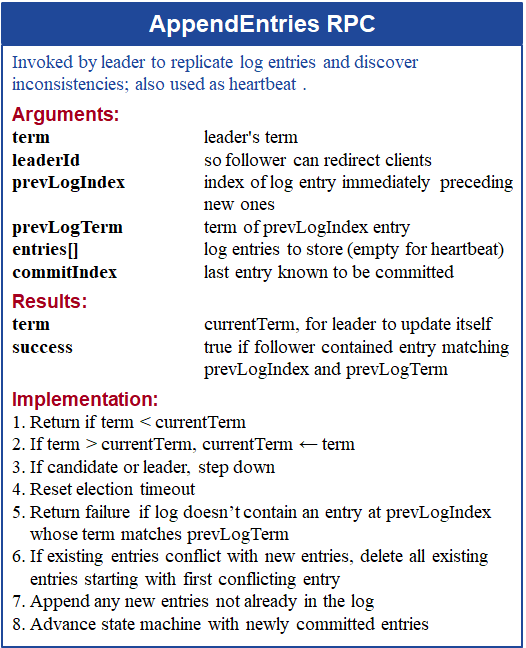
\includegraphics[width=0.99\columnwidth]{raft/appendEntries}
  	\caption{Il leader replica il proprio log inviando un elemento per volta al log dei vari follower, i quali accettano solo se c'è corrispondenza tra l'entry precedente a quella inviata dal leader e la loro ultima entry.}
  	\label{fig:figure7}
  \end{figure}

  \begin{figure}[H]
  	\centering
  	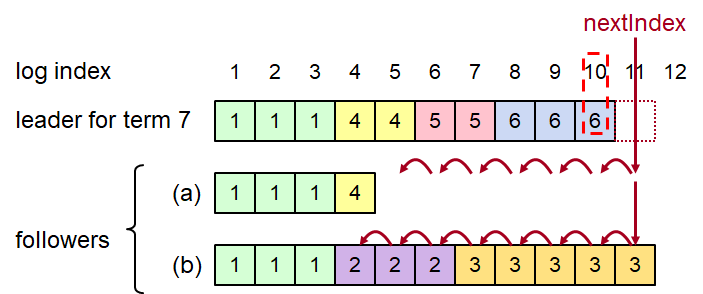
\includegraphics[width=0.99\columnwidth]{raft/repairingFollowerLogs}
    \captionsetup{singlelinecheck=off}
  	\caption[consistencyCheck2]{
    Il leader procede ad inviare entry con \textbf{indice sempre minore} fino a trovare una corrispondenza, per poi risalire fino alla cima del log, se necessario sovrascrive le entry inconsistenti del Follower.\\
  	In figura, il leader deve inviare la entry in posizione 10, con term 6.
    \begin{itemize}
      \item{\textbf{Caso a:}}
      L'indice 10 è vuoto, di conseguenza il leader procede a ritroso finché non trova \textbf{corrispondenza} all'indice 4.
      \item{\textbf{Caso b:}}
       All'indice 10 c'è una entry diversa da quella del leader, di conseguenza esso procede a ritroso fino all'indice 3, dal quale inizierà a \textbf{ricostruire il log sovrascrivendo le entry inconsistenti}.
    \end{itemize}
    }
  	\label{fig:figure8}
  \end{figure}
  Il leader continua ad inviare \textit{AppendEntries} ai followers che non rispondono, fino a quando non ottiene successo. Una eventuale presenza minoritaria di followers lenti o bloccati non intacca le performance del cluster e non rallenta la validazione di nuove entry da parte del leader.

  \subsubsection{Crash del Leader e Inconsistenze del Log}
  In situazioni normali l'algoritmo garantisce che leader e followers si mantengano consistenti e dunque il \textbf{consistency check} delle \textbf{AppendEntries} non fallisce mai.\\
  Può capitar però che il \textbf{leader crashi prima di riuscire a completare la replica sulla maggioranza dei followers}. In questo caso i log dei followers possono mostrare diversi tipi di inconsistenza (vedi figura \ref{fig:figure9}):
  \begin{itemize}
    \item{Entry mancanti}
    \item{Entry sovrabbondanti}
    \item{Entrambe le situazioni}
  \end{itemize}

  \begin{figure}[H]
    \centering
    \includegraphics[width=0.99\columnwidth]{raft/loginconsistencies}
    \caption[inconsistency]{La figura mostra un esempio in cui vengono mostrati tutti i tipi di inconsistenza possibili in RAFT.}
    \label{fig:figure9}
  \end{figure}
  In RAFT le inconsistenze sono risolte senza introdurre dei comportamenti speciali da parte del leader. Questa semplicità risiede in una importante assunzione che viene fatta dall'algoritmo: \textbf{il Leader ha pieno potere e possiede la verità assoluta.}\\
  Questa assunzione permette al leader di portare tutti i server a convergere alla propria visione del log. Questo sta a significare che i followers potrebbero addirittura \textbf{cancellare o riscrivere entry non committate} presenti nei loro log se queste non soddisfano il leader. La riparazione del log viene fatta in modo automatico tramite \textbf{AppendEntries} con \textbf{consistency check induttivo}.
		% -*- root: ../../../main.tex -*-
\subsection{Safety e Consistency}
Nelle sezioni precedenti è stato descritto il funzionamento generale di RAFT includendo alcune proprietà e vincoli essenziali per mantenere consistenza tra i log durante le principali operazioni.\\
Qui di seguito ricordiamo le proprietà nominate nelle sezioni precedenti:

\begin{itemize}
	\item{\textbf{Election Safety:}} 
  Per un dato term è possibile al più eleggere \textbf{un solo leader}.
	La dimostrazione di questa proprietà è già stata discussa precedentemente nella sezione \ref{electionsaf}.
	\item{\textbf{Leader Append-Only:}}
  Il leader non cancella \textbf{mai}, né sovrascrive le entry del proprio log.
  La proprietà è descritta in dettaglio nella sezione \ref{Log Replication}.
	\item{\textbf{Log Matching:}}
  La proprietà di log matching garantisce che:
	\begin{itemize}
		\item{\emph{Se due log hanno un entry con lo stesso index e stesso term, allora quell'entry contiene lo stesso comando(sono identiche)}}.
		\item{\emph{Se due \textit{entry} in log diversi hanno lo stesso index e lo stesso term, allora anche tutte le loro precedenti entry sono identiche tra i due log}}.
	\end{itemize}
	La proprietà è descritta in dettaglio nella sezione \ref{Log Matching}.
\end{itemize}
L'elenco sovrastante non è però completo: attualmente ci sono casi che non sono gestiti e che possono causare notevole \textbf{inconsistenza} tra i log.\\
Ad esempio se il leader \textit{valida} alcune \textit{entry} mentre un dato follower è offline, nel caso in cui il follower venisse eletto esso potrebbe sovrascrivere le entry già eseguite con quelle presenti nel proprio log.\\
E' necessario dunque completare l'algoritmo aggiungendo la proprietà chiave di tutte le state machine: la \textbf{State Machine Safety} property. 

  \paragraph{State Machine Safety}
  \emph{Se una entry è stata committata ed eseguita in una state machine, allora nessun altra state machine può committare una valore differente per la stessa entry}.\\
  la state machine safety porta all'introduzione di due \textbf{restrizioni} molto importanti all'algoritmo:
  \begin{itemize}
    \item{\textbf{Restrizione durante la leader election}}
    \item{\textbf{Restrizione nei commitment}}
  \end{itemize}


  \subsubsection{Restrizioni nelle Elezioni}
  Durante le elezioni ci sono casi in cui non è possibile determinare se un \textit{entry} è committed oppure no. Come si può vedere in figura \ref{fig:figure10} non è possibile determinare se l'ultima \textit{entry} è stata committed: per questo si aggiunge un \textbf{ulteriore vincolo all'elezione di un candidate}.
  \[
    \emph{\textbf{Scegli il candidato con il log più completo.}}
  \]

  Più precisamente il candidate invia solo le informazioni sull'\textbf{ultima entry} dato che queste informazioni definiscono interamente il log.
 \[
      AppendEntries(term, index)
  \]
  Il criterio con cui viene fatta questa valutazione è il seguente:\\
  Sia $lastTerm_v$ il term presente a indice $lastIndex_V$ della entry del log del \textbf{server votante} e $lastTerm_c$ il term presente a indice $lastIndex_C$ della entry del log del \textbf{candidate}, Allora:
  \begin{equation} \label{eq:1}
    \begin{multlined}
    Se:\\
      (lastTerm_v > lastTerm_c) \; \| \;        \\
      (lastTerm_v == lastTerm_c)  \; \&\& \;
      (lastIndex_v > lastIndex_c)
    \implies Reject
    \end{multlined}
  \end{equation}
  In altre parole:
  \begin{itemize}
    \item{\emph{Se l'ultimo term del log del server votante è maggiore di quello del server candidato, allora la  richiesta viene rifiutata. }}
    \item{\emph{Se invece i due ultimi term si equivalgono, la valutazione viene fatta tenendo conto della lunghezza del log:}}
    \begin{itemize}
      \item{\emph{Se l'ultimo indice del log di C è maggiore di quello di V la richiesta viene accettata, altrimenti viene rifiutata.}}
    \end{itemize}
  \end{itemize}
 
  \begin{figure}[H]
  	\centering
  	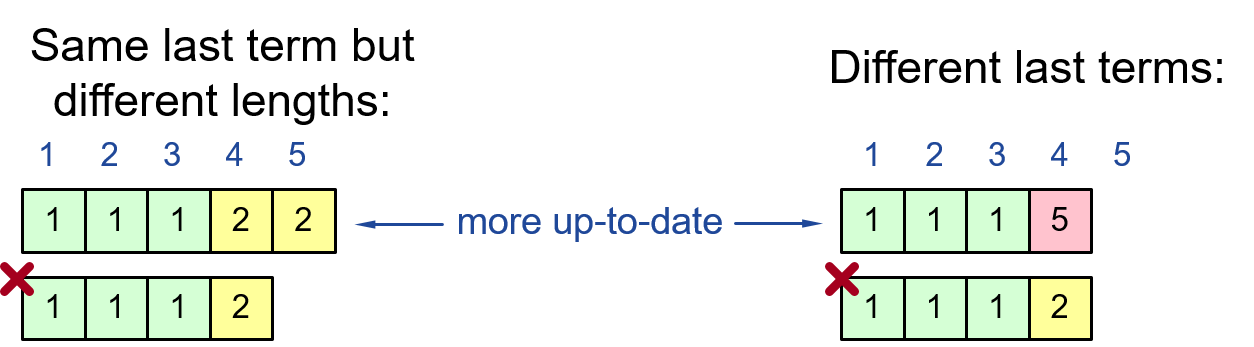
\includegraphics[width=0.99\columnwidth]{raft/pickingUpToDateLeader}
  	\captionsetup{singlelinecheck=off}
  	\caption[stateDiagramCaption]{
	 In questo caso non è possibile determinare se l'ultima \textit{entry} è validata, inoltre solo il primo server può essere eletto dato che il terzo non è disponibile.}
  	\label{fig:figure10}
  \end{figure}

  \paragraph{Commiting di Entries del term corrente}
  Vediamo ora un esempio di quello che è stato detto fino ad ora. Nella figura \ref{fig:figure11} possiamo vedere che all'indice 4 il leader $S1$ al term 2 è riuscito a \textbf{replicare con successo} la propria entry sulla maggioranza dei server; la entry è dunque \textbf{committed}. A questo punto nel caso in cui il leader $S1$ crashasse, per l'\textbf{election restriction} introdotta sopra, i server $S4$ e $S5$ non potrebbero essere eletti leader.\\
  \begin{itemize}
    \item {$S5$ non può essere eletto perché non possiede un term più piccolo di tutti gli altri $\rightarrow$ \textbf{condizione n:1}}
    \item{$S4$ non può essere eletto poiché anche se possiede un term aggiornato non ha un log completo (più corto) $\rightarrow$ \textbf{condizione n:2} }
  \end{itemize}


  \begin{figure}[H]
    \centering
    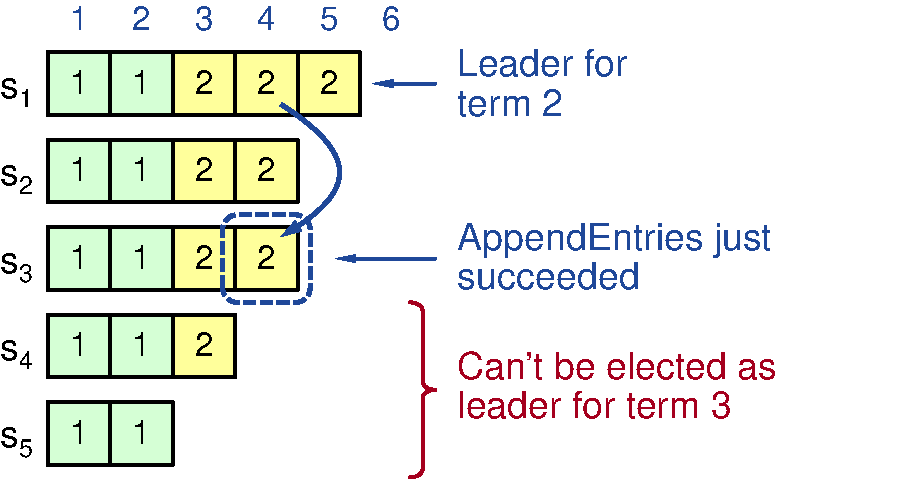
\includegraphics[width=0.99\columnwidth]{raft/committingEntryFromCurrentTerm}
    \caption[stateDiagramCaption]{$S4$ e $S5$ si trovano impossibilitati ad essere eletti come leader e quindi non sono in grado di modificare il log di latri server.}
    \label{fig:figure11}
  \end{figure}

  \subsubsection{Committing di Entries di term precedenti}
  Questo caso, descritto perfettamente nell'immagine \ref{fig:figure12} rappresenta la situazione peggiore e più inusuale per RAFT; essa si può riassumere come segue:
  \begin{enumerate}
    \item{Il server $S1$, leader al \textbf{term 2}, \textbf{replica la entry} solamente su due server e poi crasha.}
    \item{Un altro server, $S5$ viene eletto leader per il \textbf{term 3} da $S3$, $S4$ e $S5$, esso appende una serie di entry e poi crasha prima di poter comunicare.}
    \item{Il server $S1$ si risveglia e viene eletto leader da $S1$, $S2$, $S3$, $S4$ e prima di tutto cerca di \textbf{riparare} il log del sever $S3$ inviando la entry mancante.}
    \item{Il server $S5$ quando riceve gli \textbf{ack} da parte dei followers, però, \textbf{NON COMMITTA}}
    \item{Infatti, se \textbf{$S1$ crashasse dopo aver committato la entry 3} allora $S5$ potrebbe essere eletto poichè soddisfa entrambi i casi di \ref{eq:1}}
    \begin{itemize}
      \item{\textbf{Caso A}}
      \[
        lastTerm_{S5} > lastTerm_{Si} \qquad \forall i \in [2,3,4]
      \]
      \item{\textbf{Caso B}}
      \[
        lastIndex_{S5} > lastIndex_{Si} \qquad \forall i \in [2,3,4]
      \]
    \end{itemize}
    \item{Se $S5$ venisse eletto al \textbf{term 5} cercherebbe di propagare il proprio log e questo \textbf{obbligherebbe $S1$, $S2$, $S3$, e $S4$ a dover riscrivere i propri log}.\\
    \textbf{NB:} Qua abbiamo una totale mancanza di \textbf{safety}, infatti \emph{$S1$ non saprebbe cosa fare dato che le entry, una volta commitate, non possono essere cancellate dal log}}.
  \end{enumerate}
  \begin{figure}[H]
    \centering
    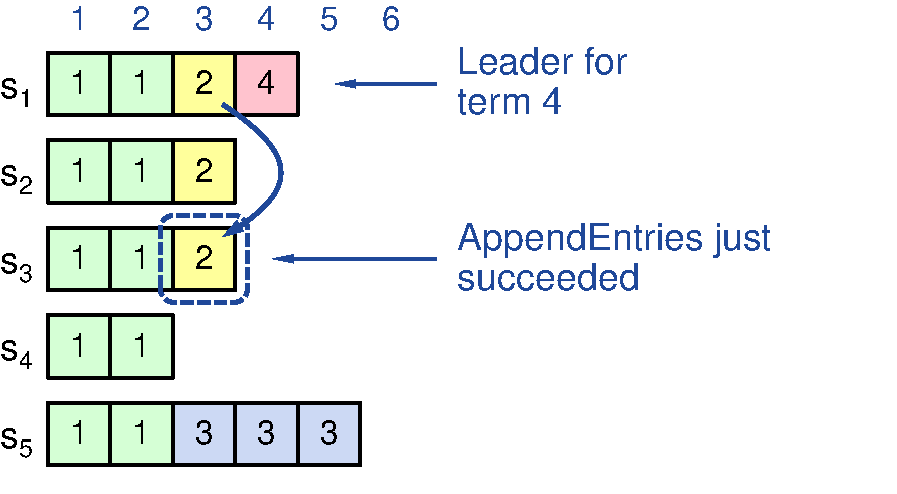
\includegraphics[width=0.99\columnwidth]{raft/committingEntryFromEarlierTerm}
    \caption[stateDiagramCaption]{}
    \label{fig:figure12}
  \end{figure}
  \paragraph{Soluzione:}
  Le regole di committing vengono estese al fine di garantire safety. Ogni leader decide se una entry è da committare in base a queste regole:
  \begin{itemize}
    \item{\emph{\textbf{La entry deve essere presente nella maggioranza dei server}}}
    \item{\emph{\textbf{Almeno una nuova entry proveniente dal leader dell'attuale term deve essere presente nella maggioranza dei server}}}
  \end{itemize}
  Come vediamo in figura \ref{fig:figure13}, nel momento in cui $S1$ viene eletto leader per il \textbf{term 4} e riesce a replicare la entry sulla maggioranza dei server, esso può finalmente \textbf{propagare le informazioni di committment} riferite a term passati.\\
  Questo garantisce che il server $S5$ non possa essere eletto leader al \textbf{term 5} per la regola 1 in \ref{eq:1}.
  \begin{figure}[H]
    \centering
    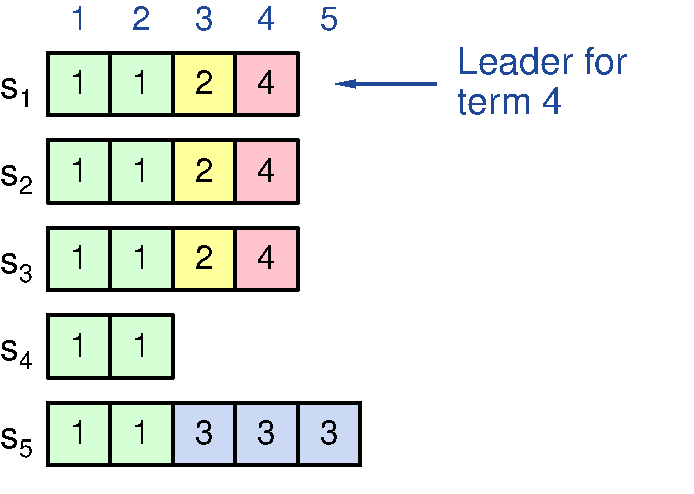
\includegraphics[width=0.80\columnwidth]{raft/newCommitmentRules}
    \caption[stateDiagramCaption]{Quando $S4$ diviene leader non committa immediatamente le entry passate ma attende l'arrivo di nuove entry. Questo evita che $S5$ possa diventare leader sovrascrivendo i logs e portando inconsistenze.}
    \label{fig:figure13}
  \end{figure}
  \subsubsection{Neutralizzazione di vecchi leader}
  Supponiamo che un leader venga momentaneamente disconnesso dalla rete, creando una cosiddetta \textbf{network partition}. RAFT essendo un algoritmo che soddisfa il requisito di \textbf{partition tolerance} garantisce che il cluster sopravviva alla failure di un membro; il cluster semplicemente eleggerà un nuovo leader.\\
  \emph{Cosa succede però se il vecchio leader torna in campo e decide di continuare a governare?}\\
  Per evitare inconsistenze RAFT mette in pratica un comportamento molto semplice, chiamato \textbf{Neutralization of stale leader}, esso funziona in modo molto semplice:
  \begin{itemize}
    \item{Ogni messaggio scambiato contiene al suo interno il \textbf{term del mittente}}.
    \item{\textbf{Caso A}}
      \[
        senderTerm > receiverTerm
      \]
      \begin{itemize}
        \item{\textbf{Il messaggio viene rifiutato.}}
        \item{\textbf{Il mittente si converte a follower.}}
      \end{itemize}
      \item{\textbf{Caso B}}
      \[
        receipTerm > senderTerm
      \]
      \begin{itemize}
        \item{\textbf{Il ricevente si converte a follower.}}
        \item{\textbf{Il ricevente aggiorna il suo term a l'ultimo ricevuto.}}
        \item{\textbf{Il ricevente processa il messaggio normalmente.}}
      \end{itemize}
  \end{itemize}
  Seguendo questi semplici casi, una volta che una \textbf{lezione} per un nuovo leader è \textbf{terminata} non è possibile che un leader deposto possa inviare messaggi alla maggioranza del cluster poiché tale maggioranza possiederà un \textbf{term aggiornato dall'ultima elezione}.
	\section{RAFT Extensions}
		% -*- root: ../../../main.tex -*-
\subsection{Client Protocol}

Il client semplicemente inviano dei comendi al leader e ricevono indietro le risposte.
se il client non sa chi è il leader va bene. Può parlare con qualsiasi macchina e se quella macchina non è il leader semplicemente dice al client chi è il leader affinchè esso possa contattarlo.


il leader non risponderà al client fino al momento in cui il comando è stato messo nel log e COMMITTATO ed eseguito dalla state machine del leader.


Che succede se il leader crasha, oppure per qualche altro motivo la richiesta scade?
- Il cliend ritrasmette il comando ad un'altra macchina. 
- Se questa macchina non è il nuovo leader, gli dice a chi rivolgersi.
- Si rivolge al nuovo leader

Questo GARANTISCE che ogni richiesta verrà gestita, PRIMA O POI.
 Ma ancora non è sufficiente a garantire che venga eseguita una e una siola volta:

può succedere che il crash del leader avvenga DOPO l'esecuzione del comando, ma PRIMA di dare la risposta al Client. 
In questo caso il client non saprebbe che il comando è stato eseguito e ritrasmetterebbe la richiesta al nuovo leader che lo porterà il quale, nel momento in cui farà commit del comando lo rieseguirà. In questo modo si avrebbe che il comando è stato eseguito due volte, il che non è accettabile.
 

Per fare ciò si introduce un identificatore univoco che viene generato dal client per ogni richiesta. 
Questo identificativo di richiesta è contenuto nella relativa entry del log.
In questo modo il leader, prima di accettare una nuova richiesta, può controllare se l'ID è già presente in una delle entry del suo log e agire di conseguenza:
 - se non è presente, lo accoda nel log e procede come di consueto
 - se è già presente, non lo accoda, ma attende che la propria state machine, se non lo ha già fatto, lo esegua; dopodichè restituisce al client il risultato.


In questo modo si garantisce che un comandovenga eseguito una e una sola volta: exactly-once semantics.

 



		% -*- root: ../../../main.tex -*-
\subsection{Configuration Changes}
La configurazione del sistema può cambiare nel tempo, ad esempio quando una macchina va incontro a crash, viene sostituita o viene aggiunta al cluster.\\

Le informazioni sulla configurazione del sistema sono cruciali perchè sapere \textbf{quanti} e \textbf{quali} server fanno parte del cluster è necessario per operazioni che necessitano di decidere basandosi sulla maggioranza, come l'elezione del leader o il commit di una entry.\\

\subsubsection{Contemporanea presenza di due configurazioni}
  Il problema che si incontra in tutti i sistemi distribuiti è che \textit{la \textbf{transizione} tra una configurazione e l'altra \textbf{non avviene nello stesso istante} per tutte le macchine}. Esisterà dunque un tempo \textbf{t} per cui \textbf{alcune} macchine saranno aggiornate sulla \textbf{nuova configurazione} mentre \textbf{altre} saranno ancora nella \textbf{vecchia}. Ciò porta a una situazione in cui è possibile che ci siano due gruppi di server, che si trovano in \textbf{due diverse configurazioni} e che rappresentano la \textbf{maggioranza} per quella configurazione.\\

  \begin{figure}[H]
    \centering
    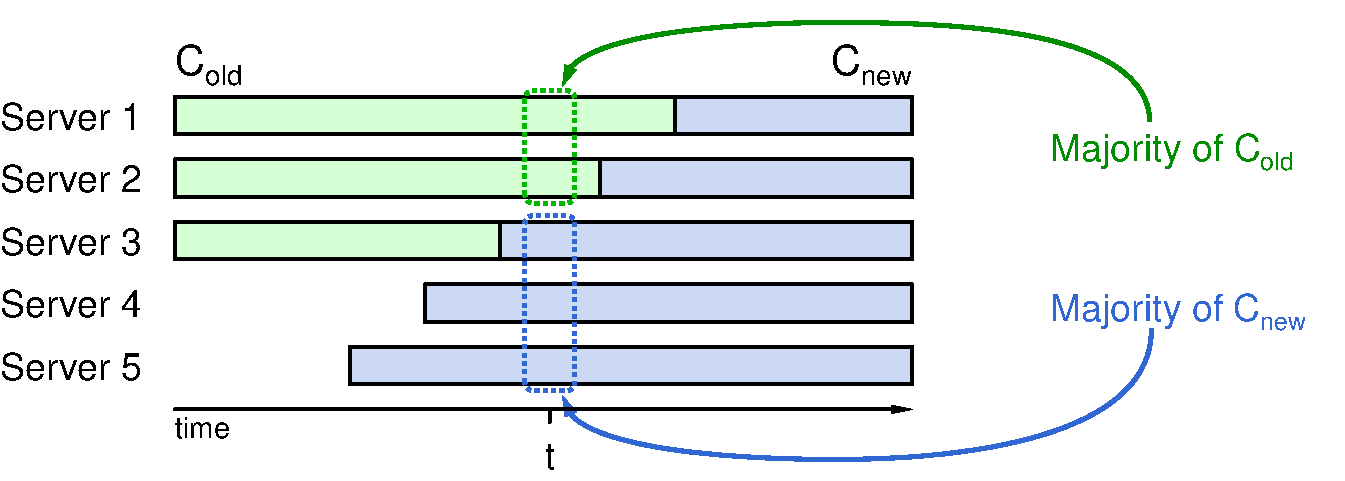
\includegraphics[width=0.90\columnwidth]{raft/configChanges.pdf}
    \caption{Esempio di \textbf{maggioranze diverse in due diverse configurazioni}: i server \textit{S4} e \textit{S5} entrano a far parte del cluster, ma al tempo \textbf{t}, si ha che \textit{S1} e \textit{S2} sono ancora alla \textbf{vecchia configurazione}, mentre \textit{S3}, \textit{S4} e \textit{S5} sono \textbf{passati alla nuova}.
    \textit{S1} e \textit{S2} costituiscono una maggioranza, nella configurazione vecchia (sono \textbf{2 su 3}), ma anche \textit{S3}, \textit{S4} e \textit{S5} possono formare una maggioranza nella loro configurazione di riferimento (\textbf{3 su 5}). }
    \label{fig:figure 8}
  \end{figure}

  \subsubsection{Problema}
    Sulla base di queste \textbf{maggioranze} possono essere portate a termine delle operazioni, come ad esempio, il commit  di una entry. Questo potrebbe generare delle \textbf{inconsistenze}, come nel caso seguente:
  \begin{enumerate}
    \item{\emph{I server \textbf{S1} e \textbf{S2} formano una \textbf{maggioranza} nella \textbf{vecchia} configurazione}}
    \item{\emph{I server \textbf{S3}, \textbf{S4} e \textbf{S5} formano una \textbf{maggioranza} nella \textbf{nuova} configurazione}}
    \item{\emph{la \textbf{maggioranza} data da S1 e S2 decide di fare \textbf{commit} dell'entry \textbf{e1}}}
    \item{\emph{la \textbf{maggioranza} data da S3,S4 e S5 decide di fare \textbf{commit} dell'entry \textbf{e2!=e1}}}
    \item{\emph{in corrispondenza dello \textbf{stesso indice}, si avranno dei \textbf{log diversi} che porteranno all'esecuzione di istruzioni diverse, generando \textbf{inconsistenza}}}
  \end{enumerate}

  Per risolvere questo problema, il passaggio tra una configurazione e l'altra non è immediato, ma viene fatto in \textbf{due fasi}.
    


  \subsubsection{Soluzione}   

    Per cambiare la configurazione del sistema, si ricorre a una \textbf{fase intermedia} posta tra la vecchia configurazione e quella nuova, in maniera tale da \textbf{evitare} di incorrere in \textbf{inconsistenze}.
    Durante questa fase intermedia, chiamata \textbf{joint consensus}, per prendere le decisioni si tengono in considerazione entrambe le maggioranze: sia quella della nuova configurazione (\textit{C\_new}) che quella della vecchia (\textit{C\_old}) in maniera tale che nè \textit{C\_old} nè \textit{C\_new} possano prendere \textbf{decisioni unilaterali}.\\

    Le caratteristiche di questo approccio sono le seguenti:
    
    \begin{itemize}
      \item{\textbf{Cambiamento della configurazione:} il passaggio a una nuova configurazione viene innescato da una richiesta. Quando il leader riceve questa richiesta la aggiunge al proprio log e la propaga, come farebbe normalmente, ma l'azione ha \textbf{effetto immediato} poichè il leader applica il cambiamento di configurazione il prima possibile, \textbf{senza attendere il commit}.}

      \item{\textbf{Configurazione intermedia:} successivamente, il leader, passa alla configurazione intermedia (\textit{C\_old+new}) e prende tutte le successive decisioni basandosi su di essa.\\
      Ad esempio, per capire se è possibile procedere con il commit di una entry, verifica che essa abbia la \textbf{\textit{maggioranza}} \textbf{sia nella vecchia} configurazione \textbf{che in quella nuova}.} 

      \item{\textbf{Decisioni sulla base di \textit{C\_old} o \textit{C\_old+new}:} esiste un periodo di tempo in cui la \textbf{entry} della nuova configurazione è \textbf{presente} nel log del leader ma \textbf{non} è ancora stata \textbf{committata}. In questo lasso di tempo è possibile che le \textbf{decisioni} possano essere prese sotto \textbf{entrambe le configurazioni}.\\ 

      Ad esempio, se il \textbf{leader} decade prima di aver \textbf{replicato} l'entry della \textbf{nuova configurazione} negli altri log, è possibile che venga eletto come \textbf{nuovo leader} un server che ha ancora la \textbf{vecchia configurazione}.\\

      Tuttavia, prima o poi arriverà un leader che non fallirà anzitempo e la nuova configurazione verrà committata. } 

      \item{\textbf{Joint consensus:} una volta fatto il \textbf{commit} diventa \textbf{impossibile} che vengano prese decisioni solo sulla base di \textit{C\_old}, perchè ora il sistema è interamente sotto la configurazione \textit{\textbf{C\_old+new}}, in uno stato di \textit{joint consensus}.
      Durante il joint consensus, la \textbf{nuova configurazione} può essere \textbf{aggiunta} al log e \textbf{propagata}.} 


      \item{\textbf{Decisioni sulla base di \textit{C\_old+new} o \textit{C\_new}:} esiste un periodo di tempo tra l'\textbf{aggiunta} nel log del leader della \textbf{nuova configurazione} e il \textbf{commit} della stessa, in cui le \textbf{decisioni} possono essere prese sulla base della configurazione \textit{\textbf{C\_old+new}} o sulla base della \textbf{nuova configurazione}. \\
      Ciò accade perchè nel caso in cui il \textbf{leader} sia soggetto a \textbf{crash}, \textbf{prima} che abbia proceduto al \textbf{commit} dell'entry relativa alla \textbf{nuova} configurazione, può essere eletto un \textbf{nuovo leader} che ha ancora la \textbf{configurazione intermedia}.\\
      Tuttavia, come nel caso precedente, si ha che \textbf{prima o poi} un leader riuscirà a fare \textbf{commit della nuova configurazione} e, da quel momento in poi, le decisioni verranno prese \textbf{solo} sulla base di quest'ultima.} 

      \item{\textbf{Elezione di leader in \textit{C\_new+old} durante\textit{ C\_new}:} non c'è \textbf{nessun momento} in cui sia \textit{C\_old} che \textit{C\_new} possono prendere \textbf{decisioni unilaterali}, generando \textbf{conflitti}. Tuttavia è possibile che anche \textbf{dopo} che \textit{C\_new} è stata \textbf{committata}, venga eletto un \textbf{leader} che \textbf{non è ancora} in tale configurazione e che quindi \textbf{non può prendere decisioni}. In questo caso esso dovrà \textbf{``dimettersi''} dando vita ad una \textbf{nuova elezione} nel momento in cui il timeout di uno degli altri follower scadrà. } 

    \end{itemize}

  \begin{figure}[H]
    \centering
    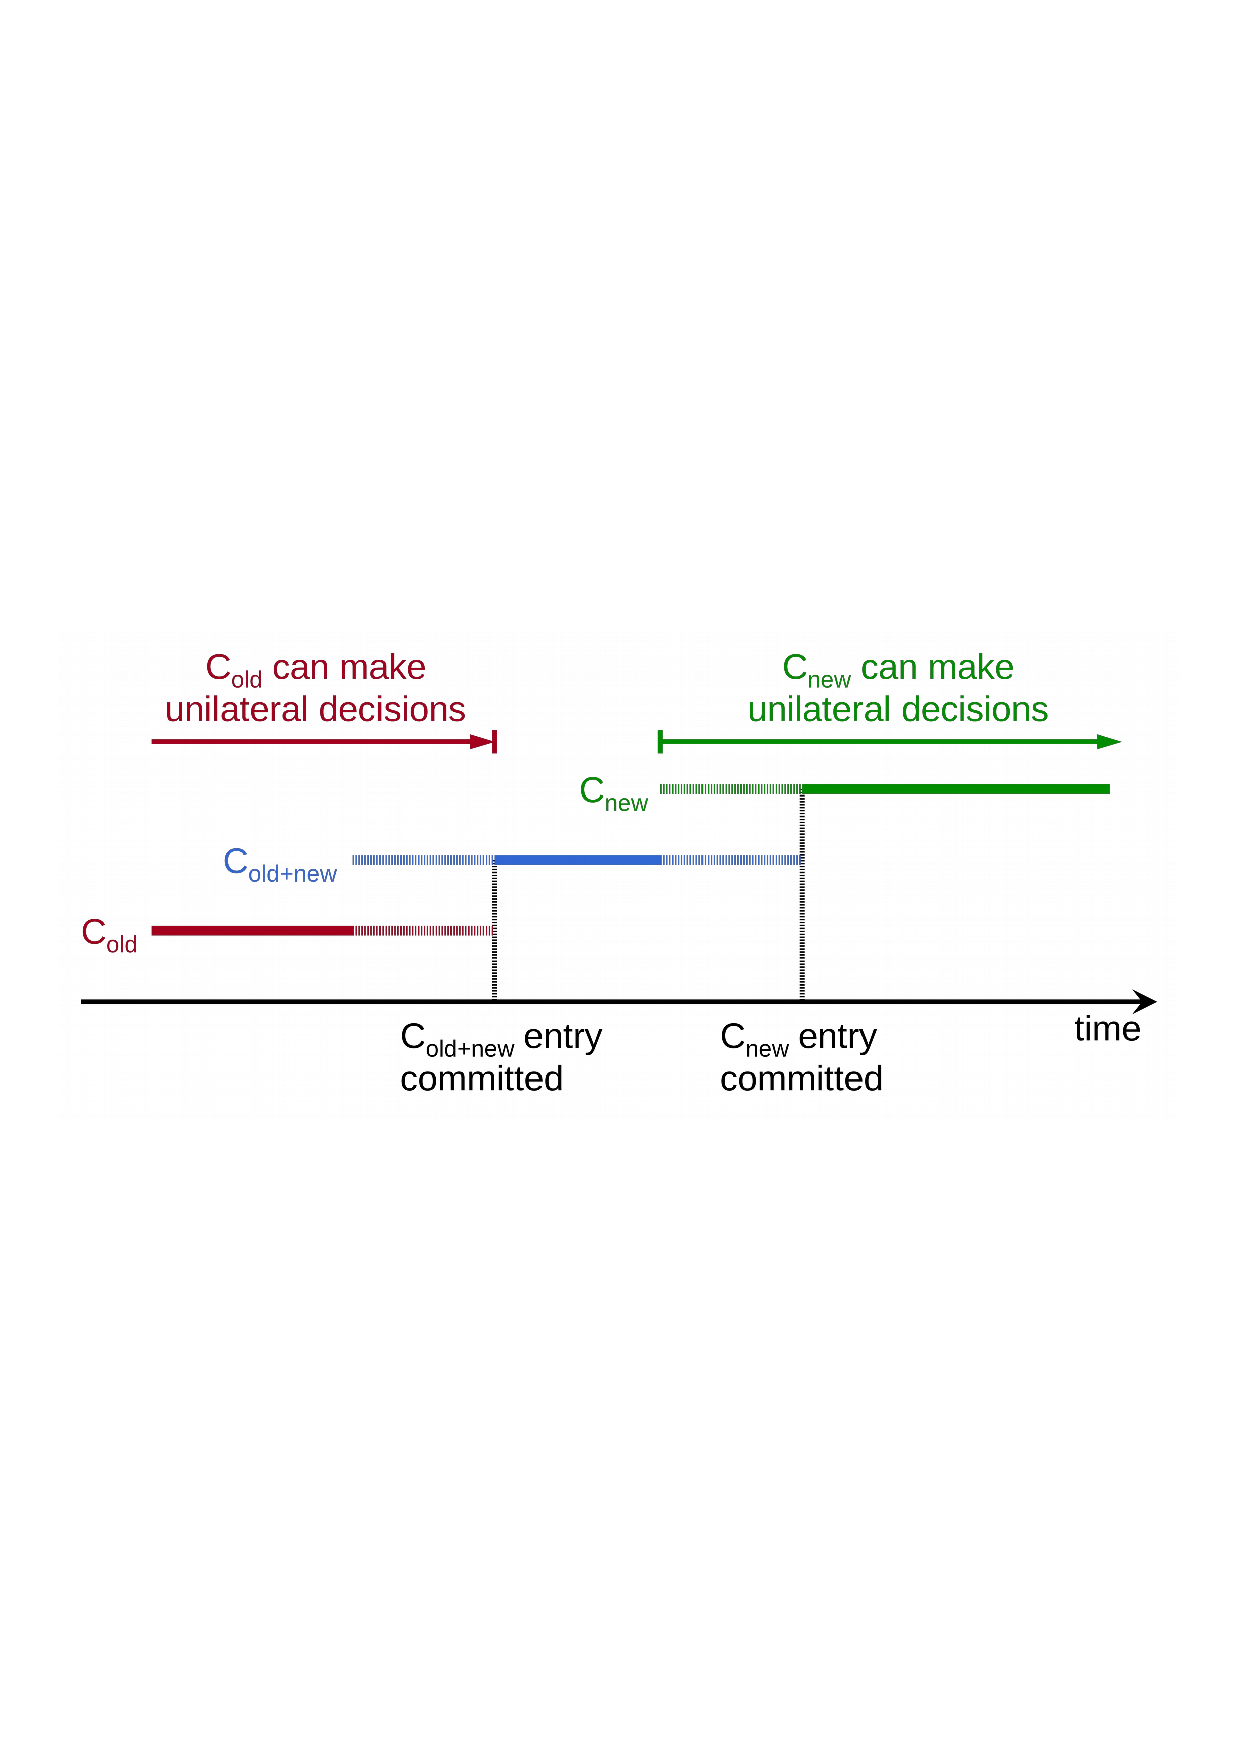
\includegraphics[width=0.90\columnwidth]{raft/jointConsensus.pdf}
    \caption{Linea temporale che mostra le fasi del passaggio del sistema da una configurazione all'altra.}
    \label{fig:figure 9}
  \end{figure}


		